\documentclass{standalone}
\begin{document}
	\subsection{Color Quantization for Medical Image Segmentation}
	

	Color quantization is the process of reducing the number of colors in a digital image. The main objective of quantization process is that 
	significant information should be preserved while reducing the number of colors in an image, in other word quantization process shouldn’t cause 
	significant information loss in the image. 
	Color quantization, accepted as a pre-processing application, is used to reduce the number of colors in images with minimum distortion such that the 
	reproduced image should be very close to the original image visually, as in \figurename\,\ref{fig:ColorQuantization}. 

	\begin{figure}[h!]
		
		\centering
			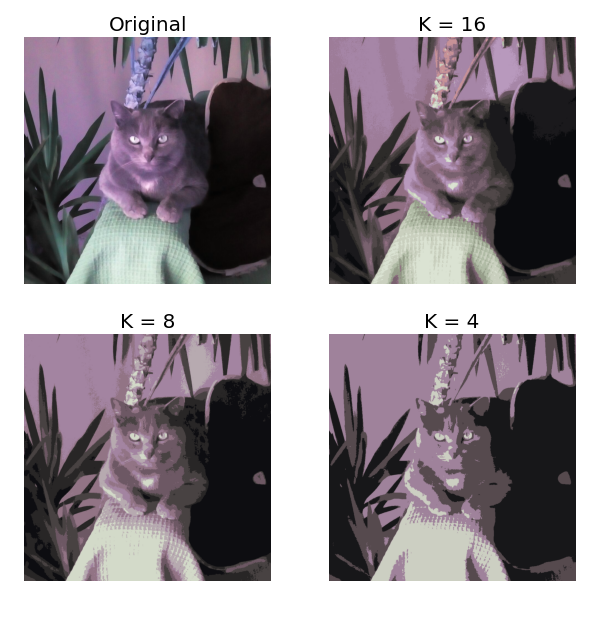
\includegraphics[scale=.6]{ColorQuantization.png}
		\caption{\textit{Color quantized RGB image. We observe the original image, a 16 color image which look similar to the original one, a 8 colors image and 4 colors image}}\label{fig:ColorQuantization}
	\end{figure}

	Color quantization play an important role in many filed of applications such as segmentation, compression, color texture analysis, watermarking, 
	text localization/detection, non photorealistic rendering and content-based retrieval~\cite{ART:Ozturk}.\\
	
	
	In this work I've applied this technique to segment CT scans of patients affected by COVID-19. Use this technique as medical image segmentation means to reduce the number of colors in the image to the number of anatomical structures and tissue present in the anatomical region; in this way we are assign to each kind of tussue a characteristic color: so must exist a relationship between the kind of tissue and the color used to represent it. 
	For CT scan which are in gray scale, each color is represented by a single value given by the Hounsfield Units(HU) : voxels colors are proportional to HU, which are defined as a linear transformation of the linear attenuation coefficient($\mu$). HU normalize the $\mu$ of a particular tissue according to a reference one, usually water($\mu_{H_2 O}$), as we can see in equation \,\ref{eq:HU} : 
	
	\begin{equation}\label{eq:HU}
		HU = k\times\frac{\mu - \mu_{H_2 O}}{\mu_{H_2 O}}
	\end{equation}
	Where $\mu_{H_20}$ is the linear attenuation coefficient of the water, $\mu$ is the linear attenuation coefficient of the tissue in the voxel and $k$ is a multiplicative constant, which can be $1000$ or $1024$ depending on the manufacturer of the CT scan.	
	In the end each color results proportional to the linear attenuation coefficient, different from each tissue, so exist a relation between the GL and the tissue type that makes this techniques available. \\
	
	Color quantization and the properties of digital images allow us to consider also other properties of the image besides the single voxel intensity.
	This purpose can be achieved by building a suitable color space: \\
	In digital image processing, images are represented with a 3D tensor, in which the first two dimensions represent the height and width of the image 
	and the last one the number of channels. Gray scale images requires only one channel, so each pixel has a numeric values whose range may change 
	according to the image format. On the other hand color images requires 3 channels, and the value of each channel represent the level of the primary 
	color stored in this particular channel, so each color is represented by 3 different values, according to Young model. \\
	In this work the different channel are used to takes in account different properties, exploited by the application of different filters. This allow us to consider also neighboring voxels, that is really suitable for the segmentation since the  lesions areas involves many closest voxels, not only a single one. We have also used this features to discriminate between other lung regions like bronchi by exploit shape information.\\
	
	Once we have build the color space, we have to found the characteristic color of each tissue under study, which is represented by a centroids in the color space. In order to perform this task and achieve the centroids estimation a simple kmeans clustering was used, since it provides a suitable segmentation with good time performances and it is efficiently implemented for multi-channel images in OpenCV~\cite{OpenCV}. 
	Kmeans clustering requires a prior knowledge about the number of cluster, which in our case is given by the anatomical structure of the lung, so we can consider a different cluster for each anatomical structure.\\
	Once we have estimated the centroids for each tissue, we use that for the actual segmentation, by assign each voxel to the cluster of the closest centroids: in this way the estimation step, that we will call "train", needs to be performed only once, so can be time expansive since is not involved in the actual segmentation.\\


	
	
	
	

	
	
\end{document}